\documentclass[11pt,a4paper]{article}
\usepackage[T1]{fontenc}
\usepackage[utf8]{inputenc}
\usepackage{lmodern}
\usepackage{microtype}
\usepackage[a4paper,margin=25mm,headheight=14pt]{geometry}
\usepackage[numbers,sort&compress]{natbib}
\usepackage{amsmath,amssymb,amsthm}
\usepackage{booktabs}
\usepackage{float}
\usepackage{graphicx}
\usepackage[font=small,labelfont=bf]{caption}
\usepackage{enumitem}
\usepackage{xcolor}
\usepackage{tikz}
\usetikzlibrary{arrows.meta,positioning}
\usepackage{fancyhdr}
\usepackage{lastpage}
\usepackage{hyperref}
\usepackage[nameinlink,noabbrev]{cleveref}
\hypersetup{colorlinks=true,linkcolor={blue!50!black},citecolor={blue!50!black},urlcolor={blue!50!black}}
\captionsetup[figure]{name=Fig.}
\setlist{nosep}
\graphicspath{{../results/figures/}}
\newtheorem{proposition}{Proposition}
\theoremstyle{definition}
\newtheorem{remark}{Remark}
\crefname{proposition}{Proposition}{Propositions}
\pagestyle{fancy}
\fancyhf{}
\lhead{\small Medical-supply depot location and helicopter routing}
\rhead{\small Page \thepage\ of \pageref*{LastPage}}
\renewcommand{\headrulewidth}{0.4pt}
\newcommand{\km}{\,\mathrm{km}}

\begin{document}

%% ================================================================== Summary
\thispagestyle{empty}
\begin{center}
{\LARGE\bfseries Location of a Medical-Supply Depot\\[3pt] and Helicopter Routing with Time-Dependent Losses\par}
\vspace{6pt}
{\normalsize Xiangyu Luo\par}
{\small Southwest Petroleum University Mathematical Modelling Contest 2023, Problem A\\ (team entry, third prize)\par}
\vspace{10pt}
{\Large\bfseries Summary\par}
\end{center}

Sichuan province plans a single depot from which transport helicopters supply the hospitals of its 21 prefecture-level units after a disaster.
Supplies deteriorate while they are on board, so the depot site, the number of helicopters and the order of their stops all affect the outcome.
We build four linked models, certify their key answers with exact optimality arguments, and test them against the parameter ranges stated in the problem.

For Problem 1 we treat the depot as the minimiser of the sum of great-circle distances to the hospitals, a spherical Weber problem.
The objective is convex but not differentiable at the hospital sites, and a real-coded genetic algorithm together with Kuhn's vertex condition shows that the optimum is exactly the Ziyang hospital, with a total distance of 3{,}847.95\,km.
The resultant of the unit vectors at Ziyang has length 0.735, so any move of the depot increases the total distance by at least 0.27\,km per kilometre, and the answer is unchanged even under a planar approximation.

For Problem 2 we formulate a capacitated, range-constrained vehicle routing problem as a mixed-integer linear programme and solve it to proven optimality for one to ten helicopters.
A single Mi-26 is infeasible because the shortest tour through all hospitals (2{,}505.5\,km) exceeds its 2{,}000\,km range, and two helicopters are optimal with 2{,}593.7\,km in total, 4.4\% shorter than the classical savings heuristic.

For Problem 3 we identify the loss law $L(t)=0.12\,(t/300)^3$, exact to the printed precision of the data, and prove that the loss-optimal plans do not depend on the cruise speed.
The distance-optimal plan loses 433\,kg, four fifths of it on the last three stops of the long south-western tour.
An $\varepsilon$-constraint model traces the distance--loss trade-off from 433\,kg down to 7.7\,kg with ten helicopters, and the compromise plan closest to the ideal point flies three helicopters over 2{,}800\,km and loses 86\,kg, an 80\% reduction for 8\% more distance.

For Problem 4 we re-solve both routing problems at 47 candidate sites.
Both transport objectives are flat around Ziyang: the best site, 18\,km to the north-west, shortens the routes by only 0.1\%, while a move to Chengdu would lengthen them by 1.1\%.
The Ziyang site is therefore appropriate.

Sensitivity analysis over the helicopter speeds, ranges and payloads given in the problem, the shape of the loss law and the parameters of the genetic algorithm shows which answers are robust and which parameters, mainly range and payload, would change the fleet size.

\medskip
\noindent\textbf{Keywords:} spherical Weber problem; Kuhn's vertex condition; vehicle routing; mixed-integer linear programming; $\varepsilon$-constraint method; emergency logistics

\newpage
\begingroup\small
\tableofcontents
\endgroup
\newpage

%% ================================================================== 1
\section{Introduction}\label{sec:intro}

\subsection{Problem Background}
The major emergencies China has faced in recent decades, among them the 1998 Yangtze floods, the SARS epidemic of 2002--2003, the snowstorms and the Wenchuan earthquake of 2008 and the COVID-19 pandemic, showed that the speed of medical logistics decides how much harm a disaster finally causes.
Sichuan, a large and mountainous province with a dense basin in the east and sparsely populated plateaus in the west, is particularly exposed, and roads are often the first infrastructure a disaster cuts.
The province therefore plans a central depot for medical supplies that serves the hospitals of all its regions by transport helicopter.

Emergency logistics of this kind combines two classical problems of operations research \citep{caunhye2012,ozdamar2004}.
The first is facility location, where the depot is placed so that the hospitals are as close to it as possible; in its simplest continuous form it is the Weber problem \citep{drezner2002}.
The second is vehicle routing, where each helicopter leaves the depot, delivers to several hospitals and returns, subject to its range and payload \citep{toth2014,laporte1992}.
What makes the present problem unusual is that the supplies lose part of their value while they are on board, and the loss grows faster than linearly with time.
The quality of a plan then depends not only on how far the helicopters fly but also on the order in which they reach the hospitals, so the location and routing decisions have to be judged by more than one criterion.

\subsection{Restatement of the Problem}
Attachment~1 gives the coordinates of one hospital in each of Sichuan's 18 prefecture-level cities and 3 autonomous prefectures, attachment~2 gives their demand for one month (12{,}000\,kg in total), and attachment~3 tabulates the loss rate of the supplies as a function of the time they have spent on board, from 10 to 300 minutes.
Transport helicopters in general fly 600--2{,}000\,km without refuelling, carry 2{,}000--12{,}000\,kg and cruise at 200--400\,km/h.
The depot operates ten Mi-26, each with a range of 2{,}000\,km, a payload of 12{,}000\,kg and a speed of 255\,km/h.
A helicopter may deliver to several hospitals on one sortie, the deliveries take no time and do not shorten the range, and after the last delivery the helicopter returns to the depot without refuelling.
On this basis the problem asks us to
\begin{enumerate}[label=(\arabic*),itemsep=2pt]
\item choose a depot site in Sichuan that minimises the total flight distance from the depot to all hospitals;
\item decide, given that depot and the demands, how many Mi-26 should be dispatched at the same time so that the total flight distance of all helicopters is minimal;
\item give a transport plan that, in addition to the flight distance, keeps the loss of supplies as small as possible;
\item judge, with all the data, whether the depot site is appropriate, and propose a new site if it is not.
\end{enumerate}

\subsection{Overview of Our Work}
The four problems form a chain in which each answer becomes an input of the next, and \cref{fig:overview} shows how our models follow it.
We begin in \cref{sec:data} with the data, which already reveal two facts that shape the later models: the total demand equals exactly one Mi-26 payload, and the farthest hospital lies only 490\,km from the centre of the province.
Model~I (\cref{sec:q1}) locates the depot by minimising the sum of great-circle distances.
Since the objective is not differentiable where the optimum turns out to lie, we do not rely on the genetic algorithm alone but prove optimality with Kuhn's vertex condition and then map how quickly the objective rises around the optimum.
Model~II (\cref{sec:q2}) takes this depot as the origin of the routes and solves the routing problem exactly for every admissible fleet size, which answers how many helicopters should fly.
Model~III (\cref{sec:q3}) first identifies the loss law hidden in attachment~3, then shows that the loss of the distance-optimal plan is concentrated on a few late stops and computes the whole range of efficient compromises between distance and loss.
Model~IV (\cref{sec:q4}) closes the loop by judging the depot with the transport objectives of Models~II and~III instead of the direct distances of Model~I.
\Cref{sec:sensitivity} tests the conclusions against the parameter ranges given in the problem, and \cref{sec:evaluation} discusses the strengths and limits of the approach.

\begin{figure}[ht]
\centering
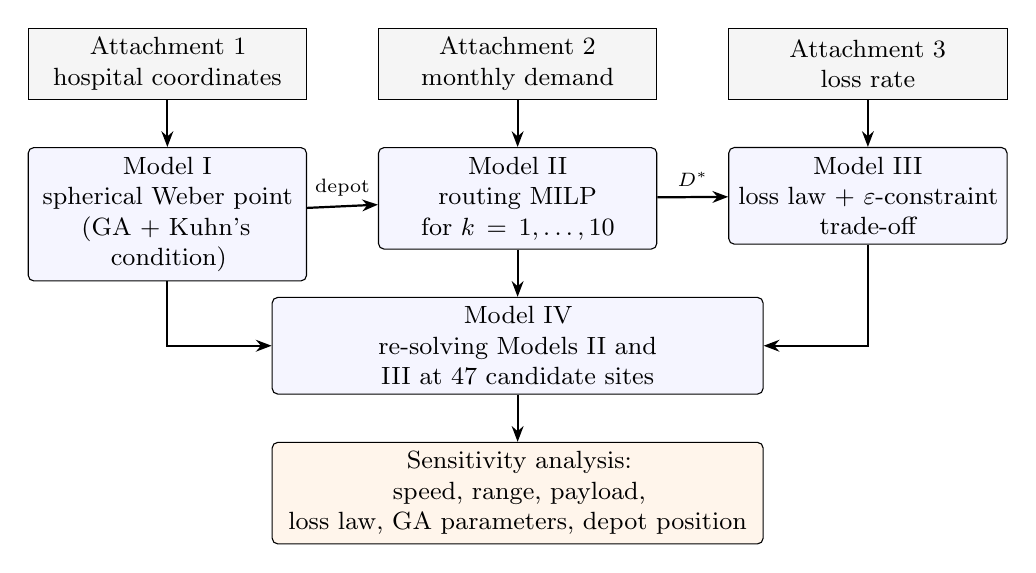
\begin{tikzpicture}[
  box/.style={draw, rounded corners=2pt, align=center, font=\small, minimum height=11mm, text width=33mm, fill=blue!4},
  data/.style={draw, align=center, font=\small, minimum height=9mm, text width=33mm, fill=gray!8},
  arr/.style={-{Stealth[length=2mm]}, thick}, node distance=6mm and 9mm]
\node[data] (a1) {Attachment 1\\hospital coordinates};
\node[data, right=of a1] (a2) {Attachment 2\\monthly demand};
\node[data, right=of a2] (a3) {Attachment 3\\loss rate};
\node[box, below=of a1] (m1) {Model I\\spherical Weber point\\(GA + Kuhn's condition)};
\node[box, below=of a2] (m2) {Model II\\routing MILP\\for $k=1,\dots,10$};
\node[box, below=of a3] (m3) {Model III\\loss law + $\varepsilon$-constraint\\trade-off};
\node[box, below=of m2, text width=60mm] (m4) {Model IV\\re-solving Models II and III at 47 candidate sites};
\node[box, below=of m4, text width=60mm, fill=orange!8] (s) {Sensitivity analysis: speed, range, payload,\\loss law, GA parameters, depot position};
\draw[arr] (a1) -- (m1);
\draw[arr] (a2) -- (m2);
\draw[arr] (a3) -- (m3);
\draw[arr] (m1) -- node[above, font=\scriptsize]{depot} (m2);
\draw[arr] (m2) -- node[above, font=\scriptsize]{$D^*$} (m3);
\draw[arr] (m1.south) |- (m4.west);
\draw[arr] (m3.south) |- (m4.east);
\draw[arr] (m2) -- (m4);
\draw[arr] (m4) -- (s);
\end{tikzpicture}
\caption{Structure of the work: the data enter the four models, each model passes its result to the next, and Model IV returns to the location question with the transport objectives.}\label{fig:overview}
\end{figure}

%% ================================================================== 2
\section{Assumptions and Justifications}\label{sec:assumptions}

The models rest on the following assumptions; each is followed by its justification and by the place where we test it.
\begin{enumerate}[label=A\arabic*.,leftmargin=*,itemsep=4pt]
\item \emph{The Earth is a sphere of radius 6{,}371\,km, and helicopters fly along great circles between sites.}
The data contain only coordinates, so terrain and air corridors cannot be modelled, and over distances of a few hundred kilometres the spherical model differs from the ellipsoid by less than 0.5\%.
In \cref{sec:q1-results} we also show that the location result survives even a crude planar approximation.
\item \emph{Each hospital receives its whole monthly demand from one helicopter, and each helicopter flies one sortie.}
Problem 2 asks how many helicopters are dispatched at the same time, and because the total demand equals one payload, splitting a hospital's delivery between helicopters can never be necessary for capacity reasons.
\item \emph{Helicopters cruise at a constant speed, delivery stops take no time and do not change the range, and there is no refuelling.}
These conditions are stated in the problem; the effect of other speeds, ranges and payloads within the admissible intervals is examined in \cref{sec:sensitivity}.
\item \emph{The loss of the supplies for a hospital depends only on the time from take-off until the helicopter reaches that hospital.}
Attachment~3 gives the loss rate as a function of time only, and all supplies are loaded at take-off.
Beyond the last tabulated time of 300 minutes we extrapolate the fitted law, and \cref{sec:sens-law} checks how much the conclusions depend on its exact shape.
\item \emph{The depot may be built anywhere in Sichuan, including at a hospital, and the hospital at the depot is supplied on the ground.}
The problem places no other restriction on the site.
If the depot coincides with a hospital, that hospital needs no flight, so its supplies suffer no in-flight loss.
\item \emph{The data in the attachments are accurate and the demand of the month is known in advance.}
The problem gives no information on uncertainty; the effect of the demand on the plans is discussed in \cref{sec:sens-range}.
\end{enumerate}

%% ================================================================== 3
\section{Notations}\label{sec:notation}

\begin{table}[ht]
\centering
\small
\begin{tabular}{ll}
\toprule
Symbol & Meaning \\
\midrule
$j=1,\dots,21$ & hospitals; node 0 is the depot \\
$a_j=(\lambda_j,\varphi_j)$ & longitude and latitude of hospital $j$ \\
$q_j$ & monthly demand of hospital $j$ (kg) \\
$z$ & depot location \\
$d(a,b)$, $d_{ij}$ & great-circle distance between points $a,b$ or nodes $i,j$ (km) \\
$F(z)$, $F^*$ & total distance from $z$ to all hospitals, and its minimum (km) \\
$S_k$ & resultant of the unit vectors at hospital $k$ pointing away from the other hospitals \\
$R_{\max}$, $Q$, $v$ & range (2{,}000\,km), payload (12{,}000\,kg), speed (255\,km/h) \\
$k$ & number of routes (helicopters) \\
$x_{ij}$ & 1 if a helicopter flies directly from node $i$ to node $j$, else 0 \\
$u_j$, $g_j$ & distance flown and load delivered when hospital $j$ is reached \\
$L(t)$ & loss rate after $t$ minutes on board \\
$\ell_j$ & loss of the supplies for hospital $j$ (kg) \\
$D^*$, $\varepsilon$ & minimum total distance of Problem 2, relative distance budget of Problem 3 \\
\bottomrule
\end{tabular}
\end{table}

%% ================================================================== 4
\section{Data Description and Preprocessing}\label{sec:data}

The 21 hospitals (\cref{tab:data} in \cref{app:data}) fall into three groups that recur throughout the paper.
Thirteen of them lie in the Sichuan basin within 160\,km of Ziyang, near its centre: Chengdu, the provincial capital, the cities of the Chengdu plain (Deyang, Mianyang, Meishan, Ya'an), of the central basin (Suining, Nanchong) and of the south (Zigong, Neijiang, Luzhou, Yibin, Leshan), and Ziyang itself.
A second group in the north-east (Guangyuan, Bazhong, Dazhou, Guang'an) lies 200--300\,km away, and a third group consists of the remote south-west and west: Panzhihua, the prefecture of Liangshan and the plateau prefectures of Garze and Aba, 250--490\,km from the centre.
The demand is uneven: Chengdu needs 2{,}000\,kg, one sixth of the total, Zigong, Mianyang and Neijiang 800\,kg each, the three autonomous prefectures 200\,kg each and every other city 500\,kg.
The total of 12{,}000\,kg equals exactly one Mi-26 payload.

Distances between two points $a=(\lambda_a,\varphi_a)$ and $b=(\lambda_b,\varphi_b)$ are computed with the haversine formula
\begin{equation}\label{eq:haversine}
d(a,b) = 2R\arcsin\sqrt{\sin^2\frac{\varphi_b-\varphi_a}{2}+\cos\varphi_a\cos\varphi_b\sin^2\frac{\lambda_b-\lambda_a}{2}}, \qquad R=6371\km ,
\end{equation}
which is numerically stable for short distances.
Two quantities follow directly from the data and bound what any plan can achieve.
Measured from the depot found in \cref{sec:q1}, the farthest hospital is Panzhihua at 489.8\,km, so a range of at least 980\,km is needed to reach every hospital with a direct return flight.
At 255\,km/h this flight takes 115 minutes, and since the loss rate grows with time, supplies for remote hospitals will always lose more than those for nearby ones.

Attachment 3 lists the loss rate every 10 minutes from 10 to 300 minutes.
The rate is zero to four decimals for the first 20 minutes, reaches 1\% after about 130 minutes and 12\% after 300 minutes, and its increments grow steadily, which already suggests a convex power law.
We identify this law in \cref{sec:q3-law}, where it is needed.

%% ================================================================== 5
\section{Model I: Depot Location (Problem 1)}\label{sec:q1}

\subsection{Model Establishment}
Problem 1 depends only on the hospital coordinates and asks for the point that minimises the total flight distance to all hospitals.
Since a flight to each hospital is counted once, the objective is
\begin{equation}\label{eq:weber}
\min_{z}\ F(z)=\sum_{j=1}^{21} d(z,a_j),
\end{equation}
the Weber (Fermat--Torricelli) problem on the sphere \citep{drezner2002,drezner1978}.
Each term $d(\cdot,a_j)$ is a geodesic distance and therefore convex along great circles as long as the points stay well inside a hemisphere; all hospitals lie within 4.5° of the province's centre, far inside the region where the spherical Weber problem is convex \citep{drezner1978}.
Hence every local minimum of $F$ is global, and we only need a reliable way to recognise one.

The difficulty lies elsewhere.
The term $d(z,a_j)$ has a cone-shaped kink at $z=a_j$, so $F$ is not differentiable at the hospital sites, and gradient-based methods such as Weiszfeld's iteration \citep{weiszfeld1937} slow down or stall when the optimum lies on a hospital.
The appropriate optimality condition at such a point is due to Kuhn \citep{kuhn1973}.
Away from $a_j$, the gradient of $d(\cdot,a_j)$ is the unit tangent vector $e_j(z)$ that points away from $a_j$, while at $z=a_k$ the term $d(\cdot,a_k)$ grows at unit rate in every direction.
For a unit tangent direction $e$ at $a_k$, the one-sided directional derivative of $F$ is therefore
\begin{equation}\label{eq:dirder}
F'(a_k;e) = 1 + \langle S_k, e\rangle, \qquad S_k = \sum_{j\neq k} e_j(a_k),
\end{equation}
and its smallest value over all directions is $1-\|S_k\|$, attained for $e=-S_k/\|S_k\|$.
Together with convexity this gives the following certificate.

\begin{proposition}[Kuhn's vertex condition]\label{prop:kuhn}
The hospital site $a_k$ minimises $F$ if and only if $\|S_k\|\le 1$.
More generally, with weights $w_j$ the condition reads $\|\sum_{j\ne k} w_j e_j(a_k)\|\le w_k$.
\end{proposition}

The vector $-S_k$ is the net ``pull'' that the other hospitals exert on a depot placed at $a_k$; the hospital itself holds the depot with a force of one, and the depot stays at $a_k$ as long as the pull does not exceed that force.
Equation \eqref{eq:dirder} also tells us more than optimality: if $\|S_k\|<1$, the total distance rises at a rate of at least $1-\|S_k\|$ in every direction, which quantifies how sharply the optimum is defined.

\subsection{Model Solution}
We solve \eqref{eq:weber} with a heuristic, a local method and the exact test, so that the three can check one another.
The heuristic is a real-coded genetic algorithm (GA) \citep{michalewicz1996}.
Each individual is a point $(\lambda,\varphi)$ in the bounding box of Sichuan ($97.35$--$108.55^\circ$E, $26.05$--$34.32^\circ$N), and its fitness is $1/F$.
The population of 100 individuals is initialised uniformly in the box and evolves for 200 generations.
In every generation parents are drawn by roulette-wheel selection on the fitness, pairs are recombined by arithmetic crossover $x'=\alpha x_a+(1-\alpha)x_b$ with probability 0.5, and each coordinate is mutated with probability 0.1 by Michalewicz's non-uniform mutation, which moves it towards a random bound by the fraction $1-r^{(1-g/G)^b}$ of the remaining distance, where $r$ is uniform on $[0,1]$, $g$ the generation, $G=200$ and $b=2$.
The mutation steps therefore shrink as the search proceeds, which turns the global exploration of the early generations into a local refinement.
The best individual is carried over unchanged (elitism).
We run the GA with 20 random seeds.

The local method is a Nelder--Mead search on $F$ started from each of the 21 hospital sites, and the exact test evaluates $\|S_k\|$ at every hospital using finite-difference gradients in local east/north coordinates (in km).

\subsection{Results}\label{sec:q1-results}
All 21 local searches converge to the Ziyang hospital site $(104.6287^\circ\text{E}, 30.1277^\circ\text{N})$ with $F^*=3{,}847.95$\,km.
The vertex test confirms this point and excludes every other hospital: at Ziyang the resultant has length $\|S_k\|=0.735<1$, whereas at the next candidates, Meishan and Chengdu, it has length 6.5 and 7.0 (\cref{tab:kuhn}).
By \cref{prop:kuhn}, Ziyang is the exact minimiser.
The 20 GA runs end on average 0.36\,km and at most 0.83\,km from it, with $F=3{,}848.06\pm0.07$\,km (mean $\pm$ s.d.), and the convergence curves in \cref{fig:q1} show the remaining excess shrinking steadily as the mutation steps contract.
The GA thus reproduces the exact solution, but it cannot by itself land precisely on a kink, which is why the certificate is needed.

\begin{table}[ht]
\centering
\caption{Kuhn's vertex test at the five hospital sites with the smallest total distance; a site is optimal if and only if $\|S_k\|\le 1$.}\label{tab:kuhn}
\small
\begin{tabular}{lrrrrr}
\toprule
 & Ziyang & Meishan & Chengdu & Neijiang & Zigong \\
\midrule
$\|S_k\|$ & 0.735 & 6.55 & 6.99 & 7.96 & 8.79 \\
$F(a_k)$ (km) & 3{,}847.95 & 4{,}073.43 & 4{,}080.32 & 4{,}164.02 & 4{,}246.80 \\
\bottomrule
\end{tabular}
\end{table}

\begin{figure}[ht]
\centering
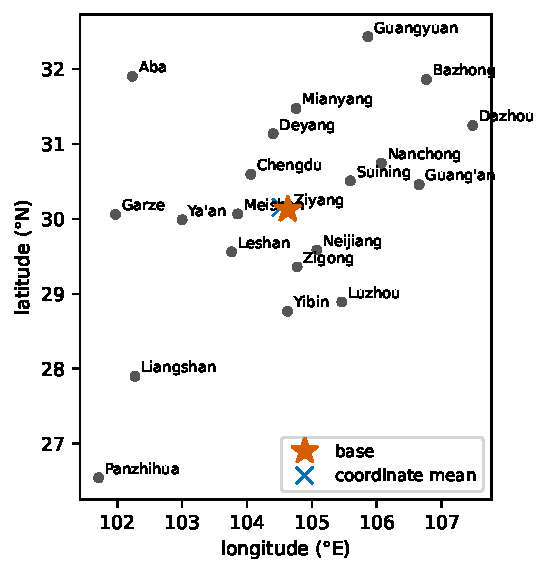
\includegraphics[width=0.49\textwidth]{q1_location}\hfill
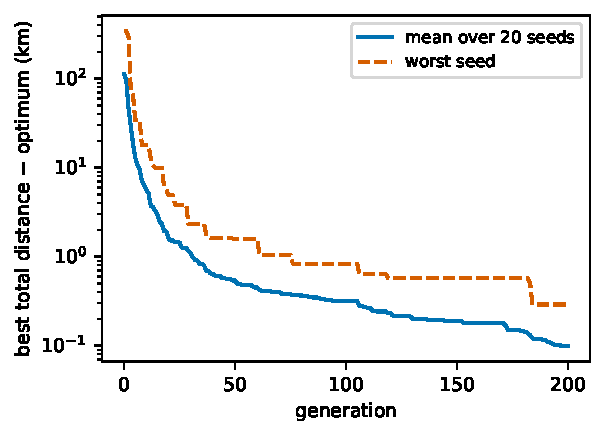
\includegraphics[width=0.46\textwidth]{q1_ga_convergence}
\caption{Left: hospitals, the optimal depot (star, Ziyang) and the arithmetic mean of the coordinates (cross). Right: convergence of the genetic algorithm over 20 seeds, measured as the excess of the best total distance over the optimum.}\label{fig:q1}
\end{figure}

The resultant at Ziyang, $S_k=(0.586,\,-0.443)$ in east/north components, also describes the shape of the objective around the optimum.
The other hospitals pull the depot towards the north-west (bearing 307°), in the direction of Chengdu and the western prefectures, but with a total force of only 0.735.
By \eqref{eq:dirder}, moving the depot by a small distance $r$ increases the total distance by between $0.265\,r$ (towards the north-west) and $1.735\,r$ (towards the south-east).
The contour map in \cref{fig:contours} and the exact values in \cref{tab:flat} confirm this first-order picture and show that, by convexity, it remains a lower bound at larger distances.
Moving the depot by 10\,km costs between 6.2 and 20.9\,km of total distance (0.2--0.5\%), and moving it by 50\,km costs between 104 and 180\,km (2.7--4.7\%).
The optimum is therefore well defined, but the objective is so flat towards the north-west that other criteria may justify a small shift in that direction; we return to this observation in \cref{sec:q4}.

\begin{figure}[ht]
\centering
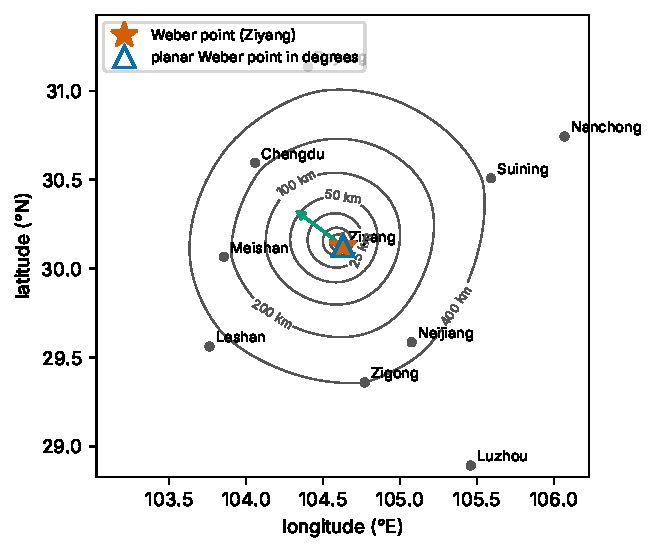
\includegraphics[width=0.62\textwidth]{q1_contours}
\caption{Excess total distance $F(z)-F^*$ around the optimum. The arrow marks the direction of the pull $-S_k$ of the other hospitals, along which $F$ rises most slowly. The planar Weber point computed in degrees (triangle) coincides with Ziyang.}\label{fig:contours}
\end{figure}

\begin{table}[ht]
\centering
\caption{Excess total distance on circles of radius $r$ around Ziyang, compared with the first-order bounds $0.265\,r$ and $1.735\,r$ from \eqref{eq:dirder}.}\label{tab:flat}
\small
\begin{tabular}{lrrrrrrr}
\toprule
$r$ (km) & 1 & 2 & 5 & 10 & 20 & 50 & 100 \\
\midrule
smallest excess (km) & 0.30 & 0.67 & 2.20 & 6.16 & 19.4 & 104 & 416 \\
largest excess (km) & 1.77 & 3.61 & 9.55 & 20.9 & 48.8 & 180 & 591 \\
$0.265\,r$ (km) & 0.27 & 0.53 & 1.33 & 2.65 & 5.30 & 13.3 & 26.5 \\
\bottomrule
\end{tabular}
\end{table}

Two simpler answers are common and worth comparing.
The arithmetic mean of the coordinates, $(104.524^\circ\text{E}, 30.153^\circ\text{N})$, lies 10.5\,km west of the optimum and has $F=3{,}855.03$\,km, 7.1\,km (0.18\%) more.
A planar Weber problem solved directly in degrees, or in an equirectangular projection, returns Ziyang as well.
This is no coincidence: the vertex condition holds with a large margin, $\|S_k\|=0.735$ against a threshold of one, so the distortions of a planar approximation are too small to move the optimum away from the vertex.
The location answer is therefore robust to the distance model, which supports assumption A1.

%% ================================================================== 6
\section{Model II: Fleet Size and Routing (Problem 2)}\label{sec:q2}

\subsection{Problem Analysis}
With the depot fixed at Ziyang, the Ziyang hospital is supplied on the ground (assumption A5) and the remaining 20 hospitals, with 11{,}500\,kg of demand, must be reached by air.
Every helicopter that flies follows a closed tour from the depot through some hospitals and back, and minimising the sum of the tour lengths is a capacitated, distance-constrained vehicle routing problem \citep{toth2014,laporte1992}.
The number of helicopters is not given but is itself the decision asked for.

Two simple bounds frame this decision.
The payload alone would allow a single helicopter, since 11{,}500\,kg is less than 12{,}000\,kg, and one tour is always the shortest way to visit all hospitals because splitting a tour forgoes the saving $d_{0i}+d_{0j}-d_{ij}\ge0$ of the triangle inequality \citep{clarke1964}.
The range, however, limits each tour to 2{,}000\,km, and whether a single tour fits depends on the length of the shortest tour through all 20 hospitals, the travelling-salesman tour.
If it does not fit, the fleet must grow, and more helicopters can only lengthen the total distance again.
The answer to Problem 2 is therefore the smallest feasible fleet, provided we can compute the optimal tours exactly; a heuristic would not tell us whether a longer total distance is due to the fleet size or to the heuristic.

\subsection{Model Establishment}
We use the two-index formulation with binary arc variables $x_{ij}$, the distance $u_j$ flown when hospital $j$ is reached and the load $g_j$ delivered up to and including $j$.
With exactly $k$ routes, the model is
\begin{align}
\min\quad & \sum_{i\neq j} d_{ij}x_{ij} \label{eq:vrp}\\
\text{s.t.}\quad & \sum_{i\neq j} x_{ij} = \sum_{i\neq j} x_{ji} = 1, && j=1,\dots,21, \label{eq:deg}\\
& \sum_{j} x_{0j} = \sum_{j} x_{j0} = k, \label{eq:k}\\
& u_j \ge u_i + d_{ij} - M(1-x_{ij}), && i,j\ge1,\ i\ne j, \label{eq:mtzu}\\
& g_j \ge g_i + q_j - Q(1-x_{ij}), && i,j\ge1,\ i\ne j, \label{eq:mtzg}\\
& d_{0j} \le u_j,\qquad u_j + d_{j0} \le R_{\max} + M(1-x_{j0}), && j\ge1, \label{eq:range}\\
& q_j \le g_j \le Q,\qquad x_{ij}\in\{0,1\}. \label{eq:load}
\end{align}
Constraints \eqref{eq:deg} require every hospital to be entered and left exactly once, and \eqref{eq:k} lets $k$ helicopters leave and return.
Constraints \eqref{eq:mtzu} propagate the flown distance along each route: if a helicopter flies from $i$ to $j$, the distance at $j$ is at least the distance at $i$ plus the leg $d_{ij}$, and with $M=R_{\max}+\max d_{ij}$ the constraint is inactive otherwise.
These distance labels also eliminate subtours, in the spirit of Miller, Tucker and Zemlin \citep{miller1960,kara2004}: a cycle $i_1\to i_2\to\dots\to i_1$ that avoids the depot would require, after summing \eqref{eq:mtzu} around the cycle, $0\ge\sum d_{i_ti_{t+1}}>0$, which is impossible because distinct hospitals are at positive distance.
Constraints \eqref{eq:range} start each route with at least the direct distance from the depot and require the distance at the last hospital plus the return leg to stay within the range, while \eqref{eq:mtzg} and \eqref{eq:load} accumulate the delivered load in the same way and cap it at the payload.
Because $u_j$ is bounded below by the true distance along the route, a feasible solution can never hide a tour that is longer than the range.

The hospital at the depot is node $j=18$ with $d_{0,18}=0$; it can be inserted next to the depot in any route at no cost, so the model needs no special treatment, and we remove it from the routes when we report them.
The model has 462 binary and 63 continuous variables and about 900 constraints.

\subsection{Model Solution}
We solve \eqref{eq:vrp} with the branch-and-cut solver HiGHS \citep{huangfu2018} for $k=1,\dots,10$ and compare the optimal distances.
For $k=1$ we first solve the travelling-salesman problem through all hospitals with the range removed: if its optimal length exceeds 2{,}000\,km, no single helicopter can be feasible, and the proven lower bound of the solver turns this into a certificate.
Every solve with $k\ge2$ terminates with a zero optimality gap.
As an independent benchmark we also run the Clarke--Wright savings algorithm \citep{clarke1964}, improved by 2-opt moves within routes \citep{lin1965} and by moves that relocate a hospital between routes.

\subsection{Results}
The optimal tour through all 20 hospitals has a length of 2{,}505.5\,km, with the lower bound of the solver equal to this value, so a single Mi-26 would exceed its range by 25\%; one helicopter is infeasible even though the payload would suffice.
With two helicopters the optimal total distance is $D^*=2{,}593.7$\,km, only 3.5\% more than the range-free tour.
The northern helicopter flies 882\,km through Chengdu, Deyang, Mianyang, Guangyuan, Bazhong, Dazhou, Guang'an, Nanchong and Suining with 6{,}300\,kg, and the southern--western helicopter flies 1{,}712\,km through Neijiang, Zigong, Luzhou, Yibin, Panzhihua, Liangshan, Garze, Aba, Ya'an, Leshan and Meishan with 5{,}200\,kg (\cref{fig:q2}, \cref{tab:route-detail} in \cref{app:routes}).
The split is natural: the eastern basin and the north-east form one compact loop, while the remote south-west and west, which cannot be added to it without exceeding the range, are combined with the southern cities that lie on the way.

\Cref{tab:q2} shows how the distance grows with the fleet.
A third route adds nothing because it is the zero-length ``route'' of the Ziyang hospital, and from then on every additional flying helicopter adds 121--214\,km, because each extra tour forgoes one of the savings that combining hospitals in a tour provides.
The payload is not binding (the loads are 6{,}300 and 5{,}200\,kg), whereas the range is the binding resource: the longer tour uses 86\% of it, and the infeasibility of $k=1$ comes from the range alone.
The depot should therefore dispatch two helicopters.

The savings heuristic finds two routes with 2{,}708.9\,km, 4.4\% more than the optimum.
It builds a western tour from Chengdu through Aba, Garze, Panzhihua and Liangshan back via Ya'an, Leshan and Meishan, and a long eastern tour through all remaining cities.
The greedy merges fix this partition early, because the savings of joining the remote prefectures are large, and the 2-opt and relocation moves cannot escape from it, whereas the optimal plan attaches the south-west to the southern cities instead.
The gap illustrates why we rely on the exact model: a heuristic answer of this quality would not reveal whether a second or third helicopter is really necessary.

\begin{table}[ht]
\centering
\caption{Minimum total flight distance with exactly $k$ routes; the route of length 0 serves the Ziyang hospital at the depot, so $k$ routes correspond to $k-1$ flying helicopters for $k\ge3$.}\label{tab:q2}
\small\setlength{\tabcolsep}{4.5pt}
\begin{tabular}{lrrrrrrrrrr}
\toprule
$k$ & 1 & 2 & 3 & 4 & 5 & 6 & 7 & 8 & 9 & 10 \\
\midrule
helicopters flying & -- & 2 & 2 & 3 & 4 & 5 & 6 & 7 & 8 & 9 \\
distance (km) & infeasible & 2{,}594 & 2{,}594 & 2{,}715 & 2{,}837 & 2{,}959 & 3{,}120 & 3{,}295 & 3{,}498 & 3{,}712 \\
longest route (km) & -- & 1{,}712 & 1{,}712 & 1{,}712 & 1{,}685 & 1{,}658 & 1{,}646 & 1{,}612 & 1{,}612 & 1{,}612 \\
\bottomrule
\end{tabular}
\end{table}

\begin{figure}[ht]
\centering
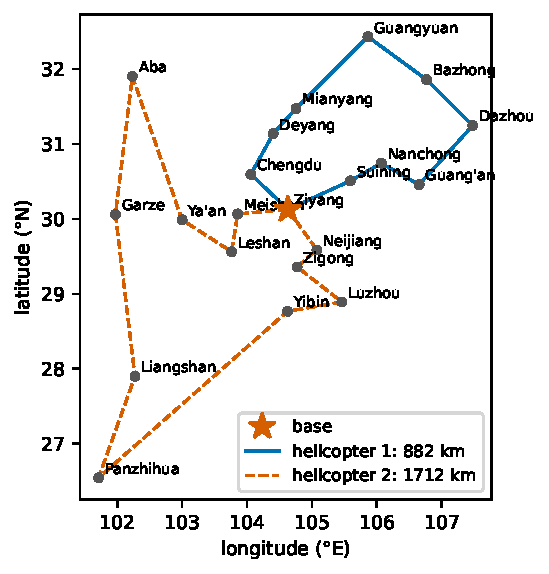
\includegraphics[width=0.62\textwidth]{q2_routes}
\caption{Distance-optimal routes of the two helicopters from the Ziyang depot.}\label{fig:q2}
\end{figure}

%% ================================================================== 7
\section{Model III: Distance--Loss Trade-off (Problem 3)}\label{sec:q3}

\subsection{Identification of the Loss Law}\label{sec:q3-law}
Before the loss can enter a model, the tabulated rates of attachment~3 must be turned into a function of time.
A power law $c\,(t/300)^p$ is the natural candidate, since the rate starts at zero and its increments grow, and a least-squares fit gives $c=0.12001$ and $p=3.0002$ with a maximum deviation of $4.5\times10^{-5}$, below the rounding of the data to four decimals.
The tabulated rates are therefore
\begin{equation}\label{eq:loss}
L(t)=0.12\left(\frac{t}{300}\right)^3 ,
\end{equation}
exactly to the printed precision (\cref{fig:loss}).
The cubic law means that deterioration accelerates: supplies that spend 100 minutes on board lose 0.44\%, those that spend 200 minutes lose 3.6\%, eight times as much.
For times beyond 300 minutes we keep the cubic law (assumption A4).

\begin{figure}[ht]
\centering
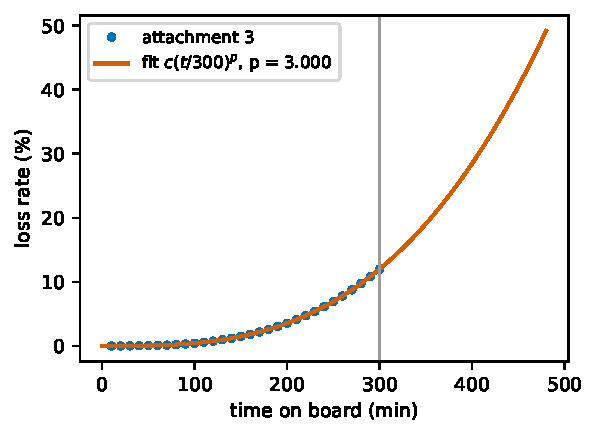
\includegraphics[width=0.5\textwidth]{q3_loss_curve}
\caption{Loss rate of attachment 3 and the fitted cubic law; the vertical line marks the end of the data.}\label{fig:loss}
\end{figure}

\subsection{Loss of a Transport Plan}
The supplies for hospital $j$ are on board from take-off until the helicopter reaches $j$, that is for $t_j=60\,u_j/v$ minutes, so their loss is
\begin{equation}\label{eq:lossj}
\ell_j = q_j\,L\!\left(\frac{60\,u_j}{v}\right) = 0.12\,q_j\left(\frac{u_j}{5v}\right)^3 ,
\end{equation}
with $u_j$ in km and $v$ in km/h.
Two consequences of \eqref{eq:lossj} shape the rest of the model.
First, the loss depends on the order of the stops through the arrival distances $u_j$, not only on the total distance: the same tour flown in the opposite direction can have a very different loss, and hospitals with large demand should be reached early.
Second, the speed enters only as a common factor.

\begin{proposition}[speed invariance]\label{prop:speed}
For any transport plan, the total loss at speed $v$ equals $(v_0/v)^3$ times the loss at speed $v_0$.
Consequently, a plan that minimises the loss subject to the range, payload and any bound on the total distance at one speed minimises it at every speed.
\end{proposition}

The proof is immediate from \eqref{eq:lossj}, because the distances $u_j$ and all constraints of \eqref{eq:vrp} are independent of the speed, and the objective $\sum_j\ell_j$ is multiplied by the constant $(v_0/v)^3$.
The speed therefore changes how much is lost but not which plan is best, a fact we use in \cref{sec:sens-speed}.

\subsection{Model Establishment}
Problem 3 asks for a plan that keeps both the flight distance and the loss small.
These objectives conflict: direct flights deliver early but multiply the distance, while long multi-stop tours keep the distance short but deliver late.
There is therefore no single best plan but a set of efficient (Pareto-optimal) plans, in which neither objective can be improved without worsening the other \citep{miettinen1999}.
We compute this set with the $\varepsilon$-constraint method \citep{haimes1971}, which minimises the loss subject to a budget on the distance,
\begin{equation}\label{eq:eps}
\min\ \sum_{j}\ell_j \quad\text{s.t. \eqref{eq:deg}--\eqref{eq:load} with } 1\le k\le 10,\qquad \sum_{i\neq j} d_{ij}x_{ij}\le(1+\varepsilon)D^*,
\end{equation}
and varies the relative budget $\varepsilon$.
Unlike a weighted sum of the objectives, this method also finds efficient plans in non-convex parts of the trade-off, which are typical of integer problems.

The cubic loss \eqref{eq:lossj} is convex in $u_j$, so it can be represented exactly by its epigraph and approximated from below by tangent planes (outer approximation \citep{duran1986}).
We add, for each hospital, the 81 cuts
\begin{equation}\label{eq:tangent}
\ell_j \ge q_j\Big(L(t_m)+L'(t_m)\big(\tfrac{60u_j}{v} - t_m\big)\Big), \qquad t_m=\frac{60}{v}\cdot\frac{m R_{\max}}{80},\quad m=0,\dots,80,
\end{equation}
which keeps the model linear.
Between two tangent points the cuts under-estimate the loss, by at most 0.11\,kg for the largest demand at the end of the range and by less than 0.03\,kg for a 500\,kg delivery within 400 minutes, and we always report the exact loss \eqref{eq:lossj} of the returned routes.
A tiny multiple ($10^{-6}$) of the distance is added to the objective to choose the shortest plan among plans with equal loss.

\subsection{Model Solution}
We solve \eqref{eq:eps} for $\varepsilon\in\{0,0.05,0.10,0.15,0.20,0.25,0.30,0.35,0.40,0.50,0.75,1.00\}$ and once without a budget.
The loss objective makes the MILP much harder than the distance problem, because the linear relaxation of the distance labels $u_j$ is weak and the cubic loss magnifies the weakness.
We therefore limit each solve to 300\,s and record the optimality gap.
Plans with a positive gap are feasible but not proven optimal, so the computed trade-off is an upper estimate of the true one; a plan returned for one budget may even be dominated by a plan found for a larger budget, and we discard such plans.
The plan without a budget is compared with a simple lower bound, the loss when every hospital is served by its own direct flight, which no plan can beat because every arrival distance is at least the direct distance.

\subsection{Results}\label{sec:q3-results}
We begin with the distance-optimal plan of Problem 2, whose loss is 433\,kg or 3.8\% of the 11{,}500\,kg of airborne supplies.
\Cref{tab:route-detail} shows where this loss arises.
The northern helicopter reaches its last hospital after 184 minutes and loses only 42\,kg, but the southern--western helicopter first flies the long loop through Panzhihua, Liangshan, Garze and Aba and reaches Ya'an, Leshan and Meishan only after 351--385 minutes.
These three cities, each with 500\,kg, lose 337\,kg together, four fifths of the total.
The direction of the tours matters as well: the plan of Problem 2 already flies both tours in the better direction, and reversing them would raise their losses from 42 to 96\,kg and from 390 to 625\,kg.
To reduce the loss substantially, the long tour has to be split.

\Cref{tab:q3} and \cref{fig:pareto} show how the efficient plans achieve this.
A distance budget of 5\% halves the loss to 226\,kg with two helicopters by reorganising the tours so that the western prefectures are visited at the end of the northern loop.
With 8\% more distance a third helicopter takes over the four southern cities, and the loss falls to 86\,kg; with 19\% more distance the three helicopters are rearranged into a western, a north-eastern and a southern tour, and the loss falls to 37\,kg.
A fourth helicopter at 24\% more distance brings it to 23\,kg and a fifth at 29\% to 15\,kg, and from there on each further reduction becomes expensive.
The loss-minimal plan uses all ten helicopters, flies 5{,}164\,km, twice the minimum, and loses 7.7\,kg (0.07\%), close to the direct-flight lower bound of 7.5\,kg (\cref{fig:minloss}).
The last column of \cref{tab:q3} expresses this pattern as the extra distance needed per kilogram saved, which is 0.6\,km/kg on the first part of the curve, rises to 6--17\,km/kg in its middle and exceeds 200\,km/kg at its end.
In other words, the first 350\,kg of loss reduction cost about 200\,km of extra flight, whereas the last 4\,kg cost more than 1{,}600\,km.

The plans for $\varepsilon=0.05$--$0.25$ stopped at the time limit with gaps of 32--92\%, while all plans from $\varepsilon=0.30$ on are proven optimal.
The large gaps mainly reflect the weak lower bounds of the formulation, but they also mean that these plans may not be optimal.
The plan found for $\varepsilon=0.15$ illustrates this: with 2{,}916\,km and 102\,kg it is dominated by the plan found for $\varepsilon=0.10$, and we exclude it from the trade-off.

\begin{table}[ht]
\centering
\caption{Efficient plans under the distance budget $(1+\varepsilon)D^*$. ``Latest'' is the latest arrival at a hospital, ``gap'' the relative MIP gap at termination (0: proven optimal), and the last column the extra distance per kilogram of loss saved relative to the previous plan. The budget $\varepsilon=1$ is not binding and gives the same plan as no budget.}\label{tab:q3}
\small
\begin{tabular}{rrrrrrr}
\toprule
$\varepsilon$ & distance (km) & loss (kg) & helicopters & latest (min) & gap & km per kg saved \\
\midrule
0 & 2{,}594 & 432.8 & 2 & 385 & 0 & -- \\
0.05 & 2{,}718 & 225.6 & 2 & 296 & 0.92 & 0.6 \\
0.10 & 2{,}800 & 86.0 & 3 & 287 & 0.77 & 0.6 \\
0.20 & 3{,}083 & 36.8 & 3 & 184 & 0.56 & 5.7 \\
0.25 & 3{,}215 & 22.7 & 4 & 155 & 0.32 & 9.4 \\
0.30 & 3{,}342 & 15.2 & 5 & 127 & 0 & 16.9 \\
0.35 & 3{,}489 & 13.0 & 5 & 118 & 0 & 67.1 \\
0.40 & 3{,}515 & 11.9 & 5 & 118 & 0 & 22.5 \\
0.50 & 3{,}864 & 10.4 & 6 & 118 & 0 & 234 \\
0.75 & 4{,}516 & 8.2 & 8 & 118 & 0 & 299 \\
1.00 & 5{,}164 & 7.7 & 10 & 118 & 0 & 1{,}344 \\
\bottomrule
\end{tabular}
\end{table}

\begin{figure}[ht]
\centering
\begin{minipage}[t]{0.48\textwidth}
\centering
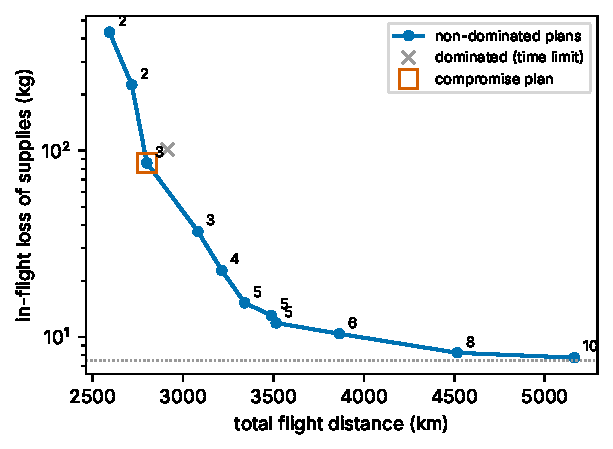
\includegraphics[width=\textwidth]{q3_tradeoff}
\caption{Distance--loss trade-off (labels: number of helicopters; square: compromise plan; cross: dominated plan; dotted line: direct-flight lower bound).}\label{fig:pareto}
\end{minipage}\hfill
\begin{minipage}[t]{0.48\textwidth}
\centering
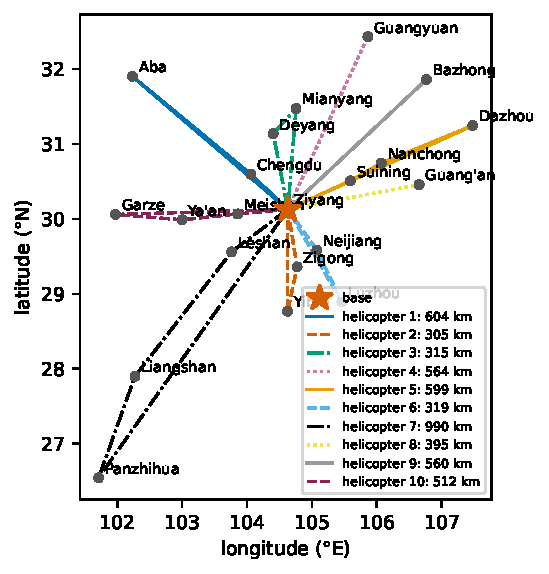
\includegraphics[width=\textwidth]{q3_routes_minloss}
\caption{Loss-minimal routes without a distance budget (ten helicopters).}\label{fig:minloss}
\end{minipage}
\end{figure}

\subsection{Choice of the Transport Plan}
A single plan must finally be recommended, and the choice depends on how a kilogram of supplies is valued against a kilometre of flight, which the problem does not specify.
We therefore use a criterion that does not need such a price, compromise programming \citep{miettinen1999}: both objectives are normalised to $[0,1]$ over the efficient set, and the plan closest to the ideal point $(0,0)$, at which both objectives would be at their best, is selected.
This plan is the three-helicopter plan with 2{,}800\,km and 86\,kg (\cref{fig:compromise}, \cref{tab:compromise-detail}), at a normalised distance of 0.201 from the ideal point.
It removes 80\% of the loss of the distance-optimal plan for 8\% more distance, and it lies at the end of the steep part of the trade-off, where the extra distance per kilogram saved starts to rise.
The northern helicopter keeps its loop, a second helicopter serves Zigong, Yibin, Luzhou and Neijiang in a short tour of 396\,km, and the third combines Meishan, Leshan and Ya'an with the remote south-west and west, reaching Liangshan after 109 minutes and Aba after 287 minutes; the two latest stops, Garze and Aba, receive only 200\,kg each, which keeps their loss small.

The criterion does not separate this plan clearly from its neighbour.
The three-helicopter plan for $\varepsilon=0.20$, with 3{,}083\,km and 37\,kg, lies at a normalised distance of 0.202, practically the same, and the four-helicopter plan follows at 0.244.
To see how the choice depends on the relative importance of the two objectives, we also minimise weighted sums of the normalised objectives.
For weights of the loss between 0.10 and 0.45 the 86\,kg plan is selected, between 0.50 and 0.60 the 37\,kg plan, between 0.65 and 0.70 the four-helicopter plan and above that the plans with five helicopters.
The 86\,kg plan is thus the choice over the widest range of weights, and we recommend it.
If the decision maker regards the loss as more important than the distance, or wants every hospital to be reached within about three hours, the three-helicopter plan with 3{,}083\,km and 37\,kg, whose latest delivery is after 184 minutes, is the better recommendation; both use three of the ten helicopters.

\begin{figure}[ht]
\centering
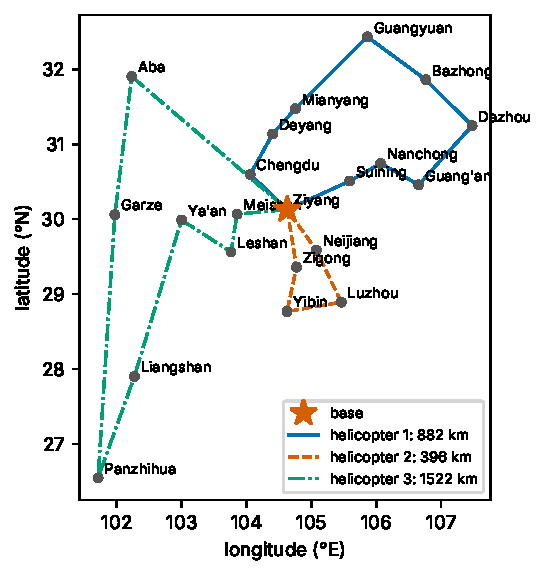
\includegraphics[width=0.62\textwidth]{q3_routes_compromise}
\caption{Compromise plan: three helicopters, 2{,}800\,km, 86\,kg of loss.}\label{fig:compromise}
\end{figure}

%% ================================================================== 8
\section{Model IV: Evaluation of the Depot Site (Problem 4)}\label{sec:q4}

\subsection{Problem Analysis}
The depot of Problem 1 minimises the sum of direct distances, with every hospital counted equally.
The transport that the depot actually performs is different in two respects: the helicopters fly multi-stop tours, whose length is not a sum of direct distances, and the hospitals differ in demand, which matters for the loss.
A site is appropriate if no other site yields clearly better transport plans, so we judge the depot by the objectives of Models II and III themselves.
\Cref{sec:q1-results} already suggests what to expect: the total direct distance rises slowly towards the north-west, so the transport objectives may favour a small shift in that direction.

\subsection{Model Establishment}
We evaluate a set of 47 candidate sites, consisting of the 21 hospital sites, the demand-weighted Weber point, which minimises $\sum_j q_j\,d(z,a_j)$ and thus accounts for Chengdu's large demand, and a regular grid of $5\times5$ points with a spacing of $0.25^\circ$ (about 24\,km in longitude and 28\,km in latitude) around Ziyang.
At every site we solve two problems: the shortest total route with any number of helicopters, that is \eqref{eq:vrp} with $1\le k\le10$, and the minimum-loss plan with up to ten helicopters, that is \eqref{eq:eps} without a budget.
The first measures how well the site supports the distance objective of Problem 2, and the second how well it supports the loss objective of Problem 3.
A site that is better in both would be a clear improvement.

\subsection{Model Solution}
Each solve is limited to 60\,s.
All 47 loss problems and the route problems at the 33 central sites are solved to optimality.
The route problems at 14 peripheral hospital sites stop with gaps of 3--30\%, but their best routes are already at least 2\% longer than at Ziyang, so the gaps cannot change the ranking.

\subsection{Results}
\Cref{fig:q4} shows that both objectives form a shallow basin around Ziyang.
The shortest routes are found at the grid point $(104.50^\circ\text{E}, 30.25^\circ\text{N})$, 18\,km north-west of Ziyang, with 2{,}591.3\,km against 2{,}593.7\,km at Ziyang, a reduction of 0.1\%.
The demand-weighted Weber point $(104.555^\circ\text{E}, 30.257^\circ\text{N})$, which lies 16\,km north-north-west of Ziyang, gives 2{,}592.4\,km.
Both lie in the direction of slowest increase found in \cref{sec:q1-results}, which confirms that Chengdu's demand and the western prefectures pull the depot gently north-west.
The minimum achievable loss is 7.73\,kg at the best grid point and 7.74\,kg at Ziyang, practically identical.
Moving the depot to Chengdu, the largest consumer, would lengthen the routes to 2{,}621.7\,km (+1.1\%) and raise the minimum loss to 8.88\,kg (+15\%), because the hospitals in the south and east would then be farther away.
Peripheral sites are much worse; at Panzhihua, for example, the routes need at least 3{,}212\,km and the loss is at least 118\,kg.

The Ziyang site is therefore appropriate.
No candidate improves either transport objective by more than 0.2\%, and the only change the data support is a move of 15--20\,km towards the north-west, which is smaller than the resolution at which a real site would be chosen.
Factors outside the data, such as available land, road access, airspace and terrain, should decide between such nearby sites.

\begin{figure}[ht]
\centering
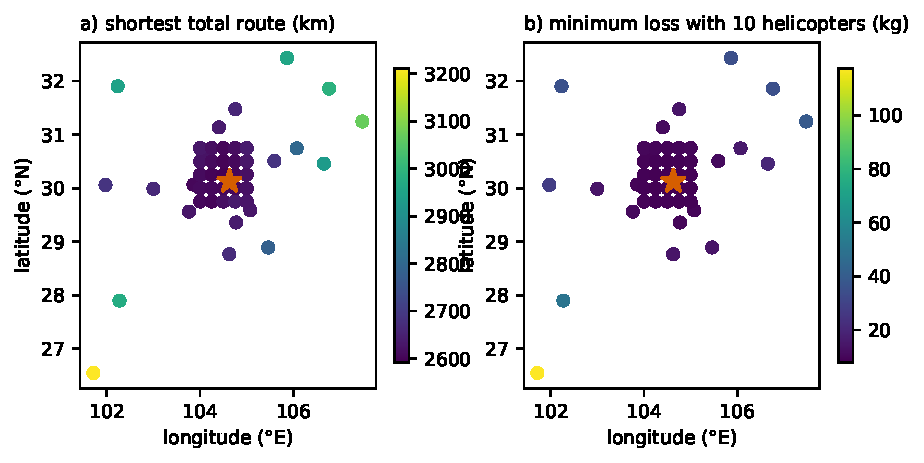
\includegraphics[width=\textwidth]{q4_candidates}
\caption{Candidate depot sites (47) coloured by a) the shortest total route length and b) the minimum in-flight loss with up to ten helicopters; star: Ziyang.}\label{fig:q4}
\end{figure}

%% ================================================================== 9
\section{Sensitivity Analysis}\label{sec:sensitivity}

The problem gives ranges rather than single values for the helicopter parameters, and the loss law beyond 300 minutes is an extrapolation.
We therefore vary each of these inputs and ask whether the answers to the four problems change.

\subsection{Helicopter Speed}\label{sec:sens-speed}
By \cref{prop:speed}, the speed does not change any optimal plan but scales every loss by $(255/v)^3$.
We confirmed this numerically by re-solving the loss-minimal problem at 200, 300 and 400\,km/h, which returned a ten-helicopter plan of the same length, 5{,}163.9\,km, each time.
\Cref{tab:speed} lists the resulting losses.
At the slowest admissible speed the distance-optimal plan would lose 897\,kg, 7.8\% of the airborne supplies, and at 400\,km/h only 112\,kg.
Since the factor is the same for every plan, the shape of the trade-off and the compromise plan are unchanged, and only the absolute losses differ.

\begin{table}[ht]
\centering
\caption{In-flight loss (kg) at different helicopter speeds; every entry equals the value at 255\,km/h times $(255/v)^3$.}\label{tab:speed}
\small
\begin{tabular}{lrrrr}
\toprule
speed (km/h) & 200 & 255 & 300 & 400 \\
\midrule
distance-optimal plan (\cref{fig:q2}) & 897 & 433 & 266 & 112 \\
compromise plan (\cref{fig:compromise}) & 178 & 86.0 & 52.8 & 22.3 \\
loss-minimal plan (\cref{fig:minloss}) & 16.0 & 7.7 & 4.8 & 2.0 \\
\bottomrule
\end{tabular}
\end{table}

\subsection{Range, Payload and Demand}\label{sec:sens-range}
The range and the payload of transport helicopters vary between 600 and 2{,}000\,km and between 2{,}000 and 12{,}000\,kg, so we re-solved Problem 2 for other values of each with the other fixed at its Mi-26 value (\cref{tab:range}).
The results follow from two bounds that the data provide.
Every hospital must be reachable by a return flight, which requires a range of at least 980\,km (\cref{sec:data}), so helicopters with a range below this value cannot serve Panzhihua from Ziyang at all, and the lower end of the admissible interval, 600\,km, is infeasible.
The payload, in turn, requires at least $\lceil 11{,}500/Q\rceil$ helicopters.

Between these bounds the fleet size is determined by whichever resource binds.
With the Mi-26 payload, a range of 1{,}000\,km needs four helicopters and 3{,}004\,km, a range of 1{,}200\,km three helicopters and 2{,}776\,km, and from 1{,}750\,km on the optimal plan of Problem 2 is feasible, since its longer tour has 1{,}712\,km.
Even a range of 2{,}500\,km would not allow a single helicopter, because the shortest tour through all hospitals is 2{,}505.5\,km.
With the Mi-26 range, a payload of 3{,}000\,kg needs four helicopters and 4{,}000\,kg three, exactly the payload bound, while from 8{,}000\,kg on the payload is no longer binding and the plan of Problem 2 is optimal.
Because a smaller range or payload only removes plans, the plan of Problem 2 stays optimal as long as it remains feasible, that is for every range from 1{,}712\,km, the length of its longer tour, up to at least 2{,}500\,km and for every payload of at least 6{,}300\,kg, its larger load.
The answer to Problem 2 is therefore stable over the upper part of both intervals, whereas helicopters with a range of 1{,}200\,km or less, or a payload of 4{,}000\,kg or less, would need three or four of them and 7--19\% more flight distance.

The same bound explains why the demand has little influence on the routes.
The loads of the two tours, 6{,}300 and 5{,}200\,kg, leave a margin of 90\% to the payload, so the demand could grow by this factor without changing the plan of Problem 2.
In Problem 3 the loss \eqref{eq:lossj} is proportional to the demand, so a uniform change of all demands scales every loss by the same factor and, as for the speed, leaves the efficient plans unchanged; only a change in the relative demands, for example a surge at a single hospital, would alter the order of the stops.

\begin{table}[ht]
\centering
\caption{Optimal fleet size and total flight distance of Problem 2 for other ranges and payloads; ``gap'' is the relative MIP gap after 180\,s (0: proven optimal).}\label{tab:range}
\small
\begin{tabular}{rrrrrr}
\toprule
range (km) & payload (kg) & helicopters & distance (km) & longest route (km) & gap \\
\midrule
600 & 12{,}000 & \multicolumn{4}{l}{infeasible (Panzhihua needs a range of 980\,km)} \\
1{,}000 & 12{,}000 & 4 & 3{,}004 & 990 & 0 \\
1{,}200 & 12{,}000 & 3 & 2{,}776 & 1{,}159 & 0.03 \\
1{,}500 & 12{,}000 & 2 & 2{,}642 & 1{,}379 & 0 \\
1{,}750 & 12{,}000 & 2 & 2{,}594 & 1{,}712 & 0 \\
2{,}000 & 12{,}000 & 2 & 2{,}594 & 1{,}712 & 0 \\
2{,}500 & 12{,}000 & 2 & 2{,}594 & 1{,}712 & 0 \\
\addlinespace
2{,}000 & 3{,}000 & 4 & 3{,}078 & 1{,}506 & 0.12 \\
2{,}000 & 4{,}000 & 3 & 2{,}827 & 1{,}159 & 0.06 \\
2{,}000 & 6{,}000 & 2 & 2{,}672 & 1{,}424 & 0 \\
2{,}000 & 8{,}000 & 2 & 2{,}594 & 1{,}712 & 0 \\
\bottomrule
\end{tabular}
\end{table}

\subsection{Shape of the Loss Law}\label{sec:sens-law}
The fitted law is exact within 300 minutes, but the distance-optimal plan delivers its last supplies after 385 minutes, so its loss depends on the extrapolation.
To test this dependence we evaluate the efficient plans under two alternative laws that agree with the data at 300 minutes, $0.12\,(t/300)^2$ and $0.12\,(t/300)^4$ (\cref{tab:law}).
The absolute losses change considerably, in particular for the plans with many helicopters, which deliver early and therefore profit most from a steeper law.
The order of the plans along the trade-off, however, is the same under all three laws for all eleven plans of \cref{tab:q3}, so the plans remain mutually non-dominated, and the qualitative recommendation, to split the long south-western tour, does not depend on the exponent.
The flatter law $p=2$ penalises the early part of every flight more and therefore reduces the benefit of additional helicopters, whereas the steeper law $p=4$ concentrates the loss on the latest deliveries and makes the first split of the long tour even more valuable: under it, the compromise plan loses only 12\% of the loss of the distance-optimal plan, against 20\% under the fitted law.

\begin{table}[ht]
\centering
\caption{Loss (kg) of the efficient plans of \cref{tab:q3} under loss laws $0.12\,(t/300)^p$ with different exponents (plans not re-optimised).}\label{tab:law}
\small
\begin{tabular}{lrrrrrrrr}
\toprule
 & \multicolumn{8}{c}{plan ($\varepsilon$)} \\
\cmidrule(l){2-9}
exponent $p$ & 0 & 0.05 & 0.10 & 0.20 & 0.25 & 0.30 & 0.50 & 1.00 \\
\midrule
2 & 429.9 & 342.1 & 151.6 & 97.3 & 64.7 & 50.1 & 39.9 & 32.1 \\
3 (fitted) & 432.8 & 225.7 & 86.0 & 36.8 & 22.7 & 15.2 & 10.4 & 7.7 \\
4 & 483.3 & 158.2 & 56.6 & 16.0 & 9.1 & 5.3 & 3.1 & 2.3 \\
\bottomrule
\end{tabular}
\end{table}

\subsection{Parameters of the Genetic Algorithm}
The GA of \cref{sec:q1} is the only stochastic component of the models.
Besides the 20 seeds of the main run, we varied the population size (50, 100, 200) and the mutation probability (0.05, 0.1, 0.2) with ten seeds each.
In all nine settings the mean distance of the final point from the optimum lies between 0.24 and 0.59\,km and the worst run ends within 1.9\,km, with the largest deviations for the small population with frequent mutation.
Since the exact answer is certified independently by \cref{prop:kuhn}, these deviations affect only the efficiency of the heuristic, not the result.

\subsection{Depot Position}
\Cref{sec:q4} doubles as a sensitivity analysis of the routing results with respect to the depot.
At the four grid points about 18\,km from Ziyang, the shortest route length changes by at most 0.4\% and the minimum loss by at most 2\%, and over the whole grid, which extends about 90\,km from Ziyang, by at most 1.7\% and 25\%.
A small error in the depot position therefore does not change the answers to Problems 2 and 3, while larger displacements mainly raise the loss, because they lengthen the flights to the far side of the province.

%% ================================================================== 10
\section{Model Evaluation and Further Discussion}\label{sec:evaluation}

\subsection{Strengths}
The main strength of the models is that their central answers are certified rather than merely found.
The depot of Problem 1 is proven optimal by Kuhn's condition, which also yields the rate at which the objective rises around it, and the routing problems of Problem 2 are solved to a zero optimality gap, with the infeasibility of a single helicopter certified by the travelling-salesman bound.
The genetic algorithm and the savings heuristic are thereby turned from answers into benchmarks, which shows how far good heuristics can be from the optimum in this setting.
The loss law recovered from attachment 3 is exact to the printed precision, and its power form leads to the speed-invariance result, which separates the questions of which plan to fly and how much will be lost.
Finally, the evaluation of the depot in Problem 4 judges the site by the same objectives as the transport plans, rather than by the direct distances of Problem 1, and the two views turn out to agree.

\subsection{Weaknesses}
The models also have limitations.
The $\varepsilon$-constrained loss problems with intermediate budgets stop at the time limit with large gaps, so the computed trade-off is an upper estimate and the true efficient plans may lose somewhat less.
Losses beyond 300 minutes rely on extrapolating the fitted law, although \cref{sec:sens-law} shows that the order of the plans does not depend on it.
Distances are great-circle distances, and mountains, weather, airspace restrictions, refuelling and loading times are ignored, as the problem prescribes; in the western plateau prefectures these factors would lengthen real flights.
The demand is treated as known, whereas after a disaster it would be uncertain and might change during the operation.

\subsection{Improvements and Extensions}
The remaining gaps could be closed by a stronger formulation of the arrival times, for example a three-index or time-indexed model, or by a branch-and-price algorithm in which each column is a route with its exact loss \citep{toth2014}.
Since the loss depends on the arrival time at every hospital, the problem is closely related to the cumulative and the time-dependent vehicle routing problems, whose specialised methods could be adapted.
Natural extensions are several sorties per helicopter, time windows for urgent hospitals, stochastic or scenario-based demand after a disaster, and a two-depot design, for example with a second depot in the west for Garze, Aba and Liangshan, whose value could be assessed with the same models.

%% ================================================================== 11
\section{Conclusions}\label{sec:conclusions}
The depot that minimises the total flight distance to the 21 hospitals is the Ziyang hospital site, with 3{,}847.95\,km in total; it is certified by Kuhn's vertex condition, and any move of the depot increases the total distance by at least 0.27\,km per kilometre.
From this depot two Mi-26 should be dispatched, since one cannot serve all hospitals within its range, and their optimal routes total 2{,}593.7\,km.
The tabulated loss rates follow $L(t)=0.12\,(t/300)^3$, under which the best plans do not depend on the speed.
The distance-optimal plan loses 433\,kg, mostly on the last stops of its long tour, and the compromise plan with three helicopters, 2{,}800\,km and 86\,kg of loss is recommended, with a rearranged three-helicopter plan (3{,}083\,km, 37\,kg) as the alternative if losses or delivery times weigh more heavily.
Re-solving the transport problems at 47 candidate sites shows that no site improves the transport objectives by more than 0.2\%, so the Ziyang site is appropriate.

%% ================================================================== References
\begingroup
\small
\begin{thebibliography}{99}
\bibitem[Caunhye et~al.(2012)]{caunhye2012} A.~M. Caunhye, X.~Nie, and S.~Pokharel. Optimization models in emergency logistics: A literature review. \emph{Socio-Economic Planning Sciences}, 46(1):4--13, 2012.
\bibitem[Clarke and Wright(1964)]{clarke1964} G.~Clarke and J.~W. Wright. Scheduling of vehicles from a central depot to a number of delivery points. \emph{Operations Research}, 12(4):568--581, 1964.
\bibitem[Drezner and Wesolowsky(1978)]{drezner1978} Z.~Drezner and G.~O. Wesolowsky. Facility location on a sphere. \emph{Journal of the Operational Research Society}, 29(10):997--1004, 1978.
\bibitem[Drezner et~al.(2002)]{drezner2002} Z.~Drezner, K.~Klamroth, A.~Sch{\"o}bel, and G.~O. Wesolowsky. The Weber problem. In Z.~Drezner and H.~W. Hamacher, editors, \emph{Facility Location: Applications and Theory}, pages 1--36. Springer, Berlin, 2002.
\bibitem[Duran and Grossmann(1986)]{duran1986} M.~A. Duran and I.~E. Grossmann. An outer-approximation algorithm for a class of mixed-integer nonlinear programs. \emph{Mathematical Programming}, 36(3):307--339, 1986.
\bibitem[Haimes et~al.(1971)]{haimes1971} Y.~Y. Haimes, L.~S. Lasdon, and D.~A. Wismer. On a bicriterion formulation of the problems of integrated system identification and system optimization. \emph{IEEE Transactions on Systems, Man, and Cybernetics}, SMC-1(3):296--297, 1971.
\bibitem[Huangfu and Hall(2018)]{huangfu2018} Q.~Huangfu and J.~A.~J. Hall. Parallelizing the dual revised simplex method. \emph{Mathematical Programming Computation}, 10(1):119--142, 2018.
\bibitem[Kara et~al.(2004)]{kara2004} I.~Kara, G.~Laporte, and T.~Bektas. A note on the lifted Miller--Tucker--Zemlin subtour elimination constraints for the capacitated vehicle routing problem. \emph{European Journal of Operational Research}, 158(3):793--795, 2004.
\bibitem[Kuhn(1973)]{kuhn1973} H.~W. Kuhn. A note on Fermat's problem. \emph{Mathematical Programming}, 4(1):98--107, 1973.
\bibitem[Laporte(1992)]{laporte1992} G.~Laporte. The vehicle routing problem: An overview of exact and approximate algorithms. \emph{European Journal of Operational Research}, 59(3):345--358, 1992.
\bibitem[Lin(1965)]{lin1965} S.~Lin. Computer solutions of the traveling salesman problem. \emph{Bell System Technical Journal}, 44(10):2245--2269, 1965.
\bibitem[Michalewicz(1996)]{michalewicz1996} Z.~Michalewicz. \emph{Genetic Algorithms + Data Structures = Evolution Programs}. Springer, Berlin, 3rd edition, 1996.
\bibitem[Miettinen(1999)]{miettinen1999} K.~Miettinen. \emph{Nonlinear Multiobjective Optimization}. Kluwer Academic Publishers, Boston, 1999.
\bibitem[Miller et~al.(1960)]{miller1960} C.~E. Miller, A.~W. Tucker, and R.~A. Zemlin. Integer programming formulation of traveling salesman problems. \emph{Journal of the ACM}, 7(4):326--329, 1960.
\bibitem[{\"O}zdamar et~al.(2004)]{ozdamar2004} L.~{\"O}zdamar, E.~Ekinci, and B.~K{\"u}{\c{c}}{\"u}kyaz{\i}c{\i}. Emergency logistics planning in natural disasters. \emph{Annals of Operations Research}, 129:217--245, 2004.
\bibitem[Toth and Vigo(2014)]{toth2014} P.~Toth and D.~Vigo, editors. \emph{Vehicle Routing: Problems, Methods, and Applications}. SIAM, Philadelphia, 2nd edition, 2014.
\bibitem[Weiszfeld(1937)]{weiszfeld1937} E.~Weiszfeld. Sur le point pour lequel la somme des distances de $n$ points donn{\'e}s est minimum. \emph{T{\^o}hoku Mathematical Journal}, 43:355--386, 1937.
\end{thebibliography}
\endgroup

%% ================================================================== Appendices
\appendix
\section{Hospital Data}\label{app:data}

\begin{table}[H]
\centering
\caption{Hospitals of the 21 prefecture-level units (attachments 1 and 2) and their great-circle distance from the Ziyang depot.}\label{tab:data}
\small
\begin{tabular}{lrrrr}
\toprule
Unit & longitude (°E) & latitude (°N) & demand (kg) & distance from depot (km) \\
\midrule
Chengdu & 104.0582 & 30.5962 & 2{,}000 & 75.6 \\
Zigong & 104.7715 & 29.3595 & 800 & 86.5 \\
Panzhihua & 101.7135 & 26.5466 & 500 & 489.8 \\
Luzhou & 105.4608 & 28.8920 & 500 & 159.3 \\
Deyang & 104.4029 & 31.1372 & 500 & 114.3 \\
Mianyang & 104.7552 & 31.4742 & 800 & 150.2 \\
Guangyuan & 105.8631 & 32.4324 & 500 & 281.8 \\
Suining & 105.5916 & 30.5083 & 500 & 101.7 \\
Neijiang & 105.0761 & 29.5855 & 800 & 74.1 \\
Leshan & 103.7624 & 29.5623 & 500 & 104.6 \\
Nanchong & 106.0687 & 30.7440 & 500 & 154.1 \\
Meishan & 103.8560 & 30.0671 & 500 & 74.6 \\
Yibin & 104.6247 & 28.7671 & 500 & 151.3 \\
Guang'an & 106.6522 & 30.4584 & 500 & 197.7 \\
Dazhou & 107.4776 & 31.2465 & 500 & 299.5 \\
Ya'an & 102.9991 & 29.9885 & 500 & 157.6 \\
Bazhong & 106.7636 & 31.8607 & 500 & 280.2 \\
Ziyang & 104.6287 & 30.1277 & 500 & 0.0 \\
Aba & 102.2324 & 31.9036 & 200 & 301.9 \\
Garze & 101.9723 & 30.0600 & 200 & 255.7 \\
Liangshan & 102.2728 & 27.8993 & 200 & 337.4 \\
\midrule
Total & & & 12{,}000 & \\
\bottomrule
\end{tabular}
\end{table}

\section{Route Details}\label{app:routes}

\begin{table}[H]
\centering
\caption{Distance-optimal plan of Problem 2: cumulative distance, arrival time, load on board before each delivery and loss of each delivery; the row of the return flight gives the total loss of the tour. The Ziyang hospital is supplied at the depot.}\label{tab:route-detail}
\small\setlength{\tabcolsep}{5pt}
\begin{tabular}{clrrrrr}
\toprule
helicopter & stop & leg (km) & cumulative (km) & arrival (min) & on board (kg) & loss (kg) \\
\midrule
1 & Chengdu & 75.6 & 75.6 & 18 & 6{,}300 & 0.05 \\
 & Deyang & 68.6 & 144.1 & 34 & 4{,}300 & 0.09 \\
 & Mianyang & 50.2 & 194.4 & 46 & 3{,}800 & 0.34 \\
 & Guangyuan & 149.3 & 343.6 & 81 & 3{,}000 & 1.17 \\
 & Bazhong & 106.0 & 449.6 & 106 & 2{,}500 & 2.63 \\
 & Dazhou & 96.1 & 545.7 & 128 & 2{,}000 & 4.70 \\
 & Guang'an & 117.8 & 663.6 & 156 & 1{,}500 & 8.46 \\
 & Nanchong & 64.2 & 727.8 & 171 & 1{,}000 & 11.16 \\
 & Suining & 52.6 & 780.4 & 184 & 500 & 13.76 \\
 & return to depot & 101.7 & 882.1 & 208 & & 42.4 \\
\addlinespace
2 & Neijiang & 74.1 & 74.1 & 17 & 5{,}200 & 0.02 \\
 & Zigong & 38.7 & 112.9 & 27 & 4{,}400 & 0.07 \\
 & Luzhou & 84.8 & 197.6 & 47 & 3{,}600 & 0.22 \\
 & Yibin & 82.6 & 280.3 & 66 & 3{,}100 & 0.64 \\
 & Panzhihua & 378.4 & 658.6 & 155 & 2{,}600 & 8.27 \\
 & Liangshan & 160.3 & 818.9 & 193 & 2{,}100 & 6.36 \\
 & Garze & 242.0 & 1{,}060.9 & 250 & 1{,}900 & 13.83 \\
 & Aba & 206.5 & 1{,}267.4 & 298 & 1{,}700 & 23.57 \\
 & Ya'an & 225.1 & 1{,}492.6 & 351 & 1{,}500 & 96.26 \\
 & Leshan & 87.6 & 1{,}580.1 & 372 & 1{,}000 & 114.22 \\
 & Meishan & 56.9 & 1{,}637.0 & 385 & 500 & 127.00 \\
 & return to depot & 74.6 & 1{,}711.6 & 403 & & 390.5 \\
\bottomrule
\end{tabular}
\end{table}

\begin{table}[H]
\centering
\caption{Compromise plan of Problem 3, in the same format as \cref{tab:route-detail}.}\label{tab:compromise-detail}
\small\setlength{\tabcolsep}{5pt}
\begin{tabular}{clrrrrr}
\toprule
helicopter & stop & leg (km) & cumulative (km) & arrival (min) & on board (kg) & loss (kg) \\
\midrule
1 & Chengdu & 75.6 & 75.6 & 18 & 6{,}300 & 0.05 \\
 & Deyang & 68.6 & 144.1 & 34 & 4{,}300 & 0.09 \\
 & Mianyang & 50.2 & 194.4 & 46 & 3{,}800 & 0.34 \\
 & Guangyuan & 149.3 & 343.6 & 81 & 3{,}000 & 1.17 \\
 & Bazhong & 106.0 & 449.6 & 106 & 2{,}500 & 2.63 \\
 & Dazhou & 96.1 & 545.7 & 128 & 2{,}000 & 4.70 \\
 & Guang'an & 117.8 & 663.6 & 156 & 1{,}500 & 8.46 \\
 & Nanchong & 64.2 & 727.8 & 171 & 1{,}000 & 11.16 \\
 & Suining & 52.6 & 780.4 & 184 & 500 & 13.76 \\
 & return to depot & 101.7 & 882.1 & 208 & & 42.4 \\
\addlinespace
2 & Zigong & 86.5 & 86.5 & 20 & 2{,}600 & 0.03 \\
 & Yibin & 67.4 & 153.9 & 36 & 1{,}800 & 0.11 \\
 & Luzhou & 82.6 & 236.5 & 56 & 1{,}300 & 0.38 \\
 & Neijiang & 85.7 & 322.2 & 76 & 800 & 1.55 \\
 & return to depot & 74.1 & 396.3 & 93 & & 2.1 \\
\addlinespace
3 & Meishan & 74.6 & 74.6 & 18 & 2{,}600 & 0.01 \\
 & Leshan & 56.9 & 131.5 & 31 & 2{,}100 & 0.07 \\
 & Ya'an & 87.6 & 219.1 & 52 & 1{,}600 & 0.30 \\
 & Liangshan & 242.8 & 461.9 & 109 & 1{,}100 & 1.14 \\
 & Panzhihua & 160.3 & 622.2 & 146 & 900 & 6.97 \\
 & Garze & 391.5 & 1{,}013.7 & 239 & 400 & 12.06 \\
 & Aba & 206.5 & 1{,}220.2 & 287 & 200 & 21.04 \\
 & return to depot & 301.9 & 1{,}522.0 & 358 & & 41.6 \\
\bottomrule
\end{tabular}
\end{table}

\section{Programs and Data}\label{app:programs}

\begin{center}
\small
\begin{tabular}{lp{0.62\textwidth}}
\toprule
File & Content \\
\midrule
\texttt{data/} & attachments 1--3 and the problem statement \\
\texttt{code/model.py} & distances, genetic algorithm, Weber point, loss fit, routing MILP (HiGHS via SciPy) \\
\texttt{code/run\_all.py} & Models I--IV with the budgets $\varepsilon\in\{0,0.05,0.10,0.25,0.50,1\}$: \cref{fig:q1,fig:q2,fig:loss,fig:minloss,fig:q4}, \cref{tab:q2} \\
\texttt{code/further\_analysis.py} & vertex test and landscape (\cref{tab:kuhn,tab:flat}, \cref{fig:contours}), route details (\cref{tab:route-detail,tab:compromise-detail}), savings heuristic, the remaining budgets and the trade-off analysis (\cref{tab:q3}, \cref{fig:pareto,fig:compromise}), sensitivity to speed, range, payload, loss law and GA parameters (\cref{tab:speed,tab:range,tab:law}) \\
\texttt{results/} & all numerical results as CSV and JSON files \\
\bottomrule
\end{tabular}
\end{center}

\end{document}
